\documentclass[border=5mm]{standalone}
\usepackage{tikz}

\begin{document}
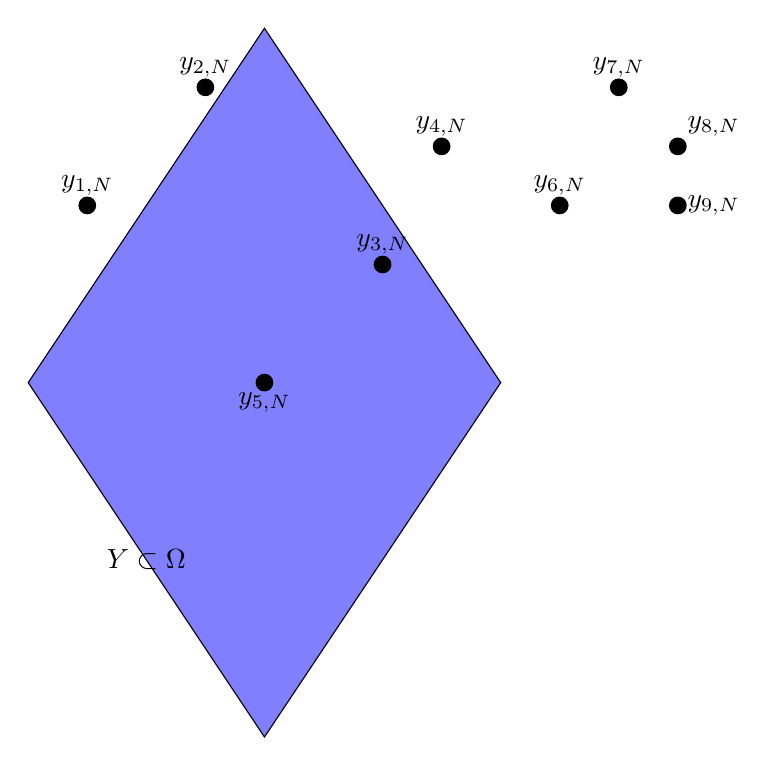
\begin{tikzpicture}[scale=1.5]
    % Define the vertices of the polygon
    \coordinate (A) at (0,0);
    \coordinate (B) at (2,3);
    \coordinate (C) at (4,0);
    \coordinate (D) at (2,-3);
    
    % Draw the polygon
    \draw[fill=blue!50] (A) -- (B) -- (C) -- (D) -- cycle;
    
    % Mark the center of the polygon
    \filldraw[black] (2,0) circle (2pt) node[below] {$y_{5,N}$};
    
    % Mark other nodes within the polygon
    \filldraw[black] (0.5,1.5) circle (2pt) node[above] {$y_{1,N}$};
    \filldraw[black] (1.5,2.5) circle (2pt) node[above] {$y_{2,N}$};
    \filldraw[black] (3,1) circle (2pt) node[above] {$y_{3,N}$};
    \filldraw[black] (3.5,2) circle (2pt) node[above] {$y_{4,N}$};
    \filldraw[black] (4.5,1.5) circle (2pt) node[above] {$y_{6,N}$};
    \filldraw[black] (5,2.5) circle (2pt) node[above] {$y_{7,N}$};
    \filldraw[black] (5.5,2) circle (2pt) node[above right] {$y_{8,N}$};
    \filldraw[black] (5.5,1.5) circle (2pt) node[right] {$y_{9,N}$};
    
    % Label the set inclusion
    \node at (1,-1.5) {$Y \subset \Omega$};
\end{tikzpicture}
\end{document}